% On découpe ce document complexe en plusieurs sous-fichiers séparés.
% Cela permettra notamment de réarranger les transparents facilement 
% lors de l'élaboration du document.

% La définition de la classe beamer avec tous les styles afférents

\RequirePackage{currfile} 

\documentclass[xcolor=table]{beamer}
\usepackage{animate}
\usepackage{colortbl}
 % Включаем поддержку UTF8  
\usepackage[russian]{babel}  

\usepackage[weather]{ifsym}

%%% Гиперссылки



%%%%%%%%%%%%%%%%%%%%%%%%%%%%%%%%%%%%%%%%%
% Beamer Presentation
% LaTeX Template
% Version 1.0 (10/11/12)
%
% This template has been downloaded from:
% http://www.LaTeXTemplates.com
%
% License:
% CC BY-NC-SA 3.0 (http://creativecommons.org/licenses/by-nc-sa/3.0/)
%
%%%%%%%%%%%%%%%%%%%%%%%%%%%%%%%%%%%%%%%%%

%----------------------------------------------------------------------------------------
%	PACKAGES AND THEMES
%----------------------------------------------------------------------------------------




\mode<presentation> {

% The Beamer class comes with a number of default slide themes
% which change the colors and layouts of slides. Below this is a list
% of all the themes, uncomment each in turn to see what they look like.

%\usetheme{default}
%\usetheme{AnnArbor}
%\usetheme{Antibes}
%\usetheme{Bergen}
%\usetheme{Berkeley}
%\usetheme{Berlin}
%\usetheme{Boadilla}
%\usetheme{CambridgeUS}
%\usetheme{Copenhagen}
%\usetheme{Darmstadt}
%\usetheme{Dresden}
%\usetheme{Frankfurt}
%\usetheme{Goettingen}
%\usetheme{Hannover}
%\usetheme{Ilmenau}
%\usetheme{JuanLesPins}
%\usetheme{Luebeck}
%\usetheme{Madrid}		
%\usetheme{Malmoe}
%\usetheme{Marburg}
%\usetheme{Montpellier}
%\usetheme{PaloAlto}
%\usetheme{Pittsburgh}
%\usetheme{Rochester}
%\usetheme{Singapore}
%\usetheme{Szeged}
\usetheme{Warsaw}

% As well as themes, the Beamer class has a number of color themes
% for any slide theme. Uncomment each of these in turn to see how it
% changes the colors of your current slide theme.

%\usecolortheme{albatross}
%\usecolortheme{beaver}
%\usecolortheme{beetle}
%\usecolortheme{crane}
%\usecolortheme{dolphin}
%\usecolortheme{dove}
%\usecolortheme{fly}
%\usecolortheme{lily}
%\usecolortheme{orchid}
%\usecolortheme{rose}
%\usecolortheme{seagull}
%\usecolortheme{seahorse}
\usecolortheme{whale}
%\usecolortheme{wolverine}

%\setbeamertemplate{footline} % To remove the footer line in all slides uncomment this line
%\setbeamertemplate{footline}[frame number] % To replace the footer line in all slides with a simple slide count uncomment this line

%\setbeamertemplate{navigation symbols}{} % To remove the navigation symbols from the bottom of all slides uncomment this line

\setbeamercovered{transparent} % Fait apparaître les animations en grisé (utile pour la conception, mais peut être commenté lors de la remise du document final)

% Pour utiliser une police à empattements partout
\usefonttheme{serif}

% Pour rajouter la numérotation des frames dans les pieds de page
\newcommand*\oldmacro{}%
\let\oldmacro\insertshorttitle%
\renewcommand*\insertshorttitle{%
  \oldmacro\hfill%
  \insertframenumber\,/\,\inserttotalframenumber}

}

\usepackage{graphicx} % Allows including images
\usepackage{booktabs} % Allows the use of \toprule, \midrule and \bottomrule in tables




% Les autres packages utiles  notamment pour le français, les accents ou Python
\usepackage{natbib}         % Pour la bibliographie
\usepackage{url}            % Pour citer les adresses web
\usepackage[T1]{fontenc}    % Encodage des accents
\usepackage[utf8]{inputenc} % Lui aussi
\usepackage[frenchb]{babel} % Pour la traduction française


\usepackage{amsmath}        % La base pour les maths
\usepackage{mathrsfs}       % Quelques symboles supplémentaires
\usepackage{amssymb}        % encore des symboles.
\usepackage{amsfonts}       % Des fontes, eg pour \mathbb.

\usepackage{cancel}

%\usepackage[svgnames]{xcolor} % De la couleur

%%% Si jamais vous voulez changer de police: décommentez les trois 
%\usepackage{tgpagella}
%\usepackage{tgadventor}
%\usepackage{inconsolata}

%%% Pour L'utilisation de Python
\usepackage{minted}
\usemintedstyle{friendly}

\usepackage{graphicx} % inclusion des graphiques
\usepackage{wrapfig}  % Dessins dans le texte.

\usepackage{tikz}     % Un package pour les dessins (utilisé pour l'environnement {code})
\usepackage[framemethod=TikZ]{mdframed}

% Les macros et raccourcis personnels
% Ce fichier contient toutes les macros que vous pouvez avoir envie de définir 
% si vous les utilisez plusieurs fois dans le document.

\PassOptionsToPackage{svgnames}{color}

% Un environnement pour bien présenter le code informatique
\newenvironment{code}{%
\begin{mdframed}[linecolor=green,innerrightmargin=30pt,innerleftmargin=30pt,
backgroundcolor=black!5,
skipabove=10pt,skipbelow=10pt,roundcorner=5pt,
splitbottomskip=6pt,splittopskip=12pt]
}{%
\end{mdframed}
}

% Un raccourci pour composer les unités correctement (en droit)
% Exemple: $v = 10\U{m.s^{-1}}$

% Les guillemets \ofg{par exemple}
\newcommand{\ofg}[1]{\og{}#1\fg{}}

% Le d des dérivées doit être droit: \frac{\dd x}{\dd t}
\newcommand{\dd}{\text{d}}

% La dérivée temporelle, tellement courante en physique, avec les d droits
\newcommand{\ddt}[1]{\frac{\dd #1}{\dd t}}

% Des parenthèses, crochets et accolades qui s'adaptent automatiquement à la 
% taille de ce qu'il y a dedans
\newcommand{\pa}[1]{\left(#1\right)}
\newcommand{\pac}[1]{\left[#1\right]}
\newcommand{\paa}[1]{\left\{#1\right\}}

% Un raccourci pour écrire une constante
\newcommand{\cte}{\text{C}^{\text{te}}}

% Pour faire des indices en mode texte (comme les énergie potentielles)
\newcommand{\e}[1]{_{\text{#1}}}

% Le produit vectoriel a un nom bizarre:
\newcommand{\vectoriel}{\wedge}


% On définit le titre et l'auteur du document

% L'argument optionnel (entre crochets) donne le titre qui sera mis sur chaque slide
\title[Multi-step forecasting]{Модель многошагового прогнозирования динамики цен мировых товарных рынков}
\author{Зехов Матвей\\
\and Николай Пильник}
% Votre nom
% L'épreuve (car on n'a pas le droit de signaler sa provenance à un concours) (là encore, l'argument optionnel apparaît sur chaque slide)
\institute[HSE]{Высшая Школа Экономики}
\date{2020} 

% On démarre le document proprement dit
\begin{document}

% La page de titre et la table des matières
% Rien d'autre à faire qu'afficher le titre
\begin{frame}
\titlepage 
\end{frame}

\begin{frame}
\frametitle{Какой товар?}
\begin{enumerate}[\Sun]
	\item Товары первого уровня: нефть, газ, золото...
	
	\item Товары второго уровня: аммиак, карбонилы...
	
	\item Усложнение задачи по сравнению с товарами первого уровня (переработка, зависимость от товаров первого уровня, ...)
	
	\item Цен много, что делать? - Использовать базисные цены.
	
	\item Разветвлённая товарная сеть товара второго уровня
	
	\item Общие тренды, следовательно, при прогнозе одного порта можно учитывать другие.
\end{enumerate}
\end{frame}

\begin{frame}
\frametitle{Описание данных}
\begin{table}[]
	\begin{tabular}{|c|c|}
		\hline
		Товар                 & Аммиак         \\ \hline
		Количество "портов"   & 9              \\ \hline
		Тип данных            & Временные ряды \\ \hline
		Периодичность         & Неделя         \\ \hline
		Старт                 & 04.07.2004     \\ \hline
		Финиш                 & 12.01.2020     \\ \hline
		Количество наблюдений & 811            \\ \hline
	\end{tabular}
\end{table}

\end{frame}



\begin{frame}
\frametitle{Примеры рядов}

\begin{center}
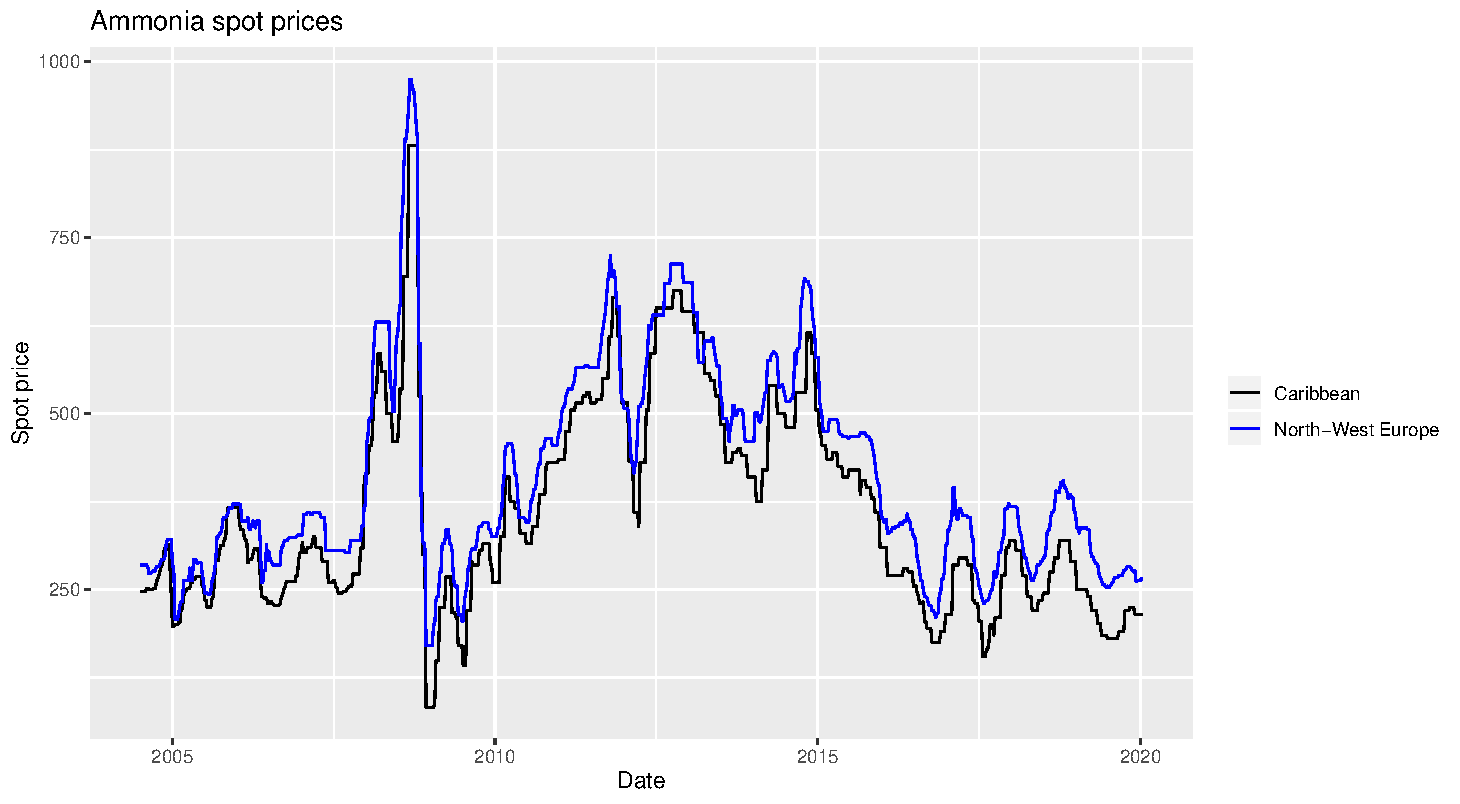
\includegraphics[width = \linewidth]{slides/series.pdf}
\end{center}
\end{frame}

\begin{frame}
\frametitle{Задачи}

\begin{enumerate}[\Sun]
\item Научиться прогнозировать цену в определённом формате на определённый горизонт для каждого порта
\item Протестировать методы и разные подходы, сопоставить точность прогнозов
\item На выходе получить набор некоторых утверждений, позволяющих строить прогноз на каждом порту.
\end{enumerate}
\end{frame}

\begin{frame}
\frametitle{Структура}
\begin{enumerate}
	\item Какой набор экзогенных переменных взять?
	
	\item Какова функциональная форма модели (абсолютные, разности, темпы)?
	
	\item Учёт динамики и глубина прогноза?
	
	$ \hat{y}_i = \alpha y_{i-1} + \beta $ или $ \hat{y}_i = \alpha \hat{y}_{i-1} + \beta $
	
	\item Критерий качества оценки модели?
	
	\item Критерий качества прогноза модели и трактуем ли он?
	
\end{enumerate}
\end{frame}


\begin{frame}
\frametitle{Критерий качества оценки модели}
\begin{enumerate}
	\item Характеристики метрики? BDP, bounded influence function, asympthotic efficiency, reaction to non-normality
	
	\item BDP
	
	\item Ограниченная influence function
	
	\item Реакия на ненормальность остатков
	
	\item Эффективность относительно OLS
	
	\item Реакция на ненормальность остатков
	
	
\end{enumerate}
\end{frame}




% La première grande partie: introduction du sujet

\end{document}


